\raggedbottom

\chapter{Implementación}
\section{Implementación del backend}
El backend de una aplicación web es la parte que se encarga de gestionar la lógica de negocio,
la comunicación con la base de datos y la API REST que se utiliza para interactuar con el frontend.
Su desarrollo se ha realizado utilizando el framework \texttt{Express.js} de \texttt{Node.js},
que permite crear aplicaciones web de manera sencilla y rápida.

\subsection{Estructura de carpetas}
\begin{figure}[H]
    \centering
    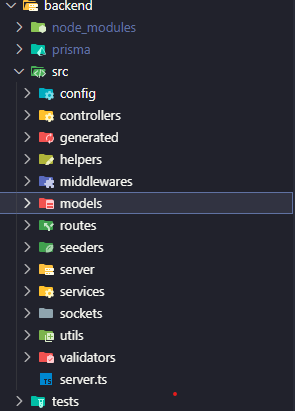
\includegraphics[width=0.7\textwidth]{imagenes/Implementacion/estructuraCarpetasBackend.png}
    \caption{Estructura de carpetas del backend}
    \label{fig:estructura_backend}
\end{figure}

\begin{itemize}
\item \textbf{\texttt{src/services}}: lógica de negocio. Contiene casos de uso (crear remesa, consultar trazabilidad, verificar autenticidad, etc.). No conoce Express: trabaja con tipos de dominio y delega el acceso a datos.
\item \textbf{\texttt{src/controllers}}: controladores. Reciben las peticiones HTTP, validan los datos y llaman a los servicios correspondientes. Conocen Express y son responsables de la serialización de las respuestas.
\item \textbf{\texttt{src/routes}}: definición de las rutas de la API. Utilizan los controladores para gestionar las peticiones y respuestas.
\item \textbf{\texttt{src/middlewares}}: middlewares de Express. Se encargan de tareas como la autenticación.
\item \textbf{\texttt{src/models}}: modelos de datos. Definen la estructura y tipo de los datos.
\item \textbf{\texttt{src/sockets}}: lógica de comunicación en tiempo real mediante WebSockets.
\item \textbf{\texttt{src/helpers}}: funciones de ayuda para tareas comunes.
\item \textbf{\texttt{src/validators}}: validadores de datos de entrada. 
\item \textbf{\texttt{src/server}}: configuración de respuesta de errores.
\item \textbf{\texttt{src/seeders}}: scripts para poblar la base de datos con datos iniciales.
\item \textbf{\texttt{src/generated y src/config}}: archivos de configuración del ORM y de las tablas de la base de datos.
\end{itemize}

\subsection{API REST}
La API REST del backend se ha diseñado siguiendo los principio RESTFul, utilizando los métodos HTTP adecuados para cada operación.
\begin{itemize}
\item \textbf{GET}: para obtener datos.
\item \textbf{POST}: para crear nuevos recursos.
\item \textbf{PUT}: para actualizar recursos existentes.
\item \textbf{DELETE}: para eliminar recursos.
\item \textbf{PATCH}: para actualizaciones parciales de recursos.
\end{itemize}

\subsubsection{Principales endpoints}
A continuación, se describen algunos de los principales endpoints de la API REST del backend:
\begin{itemize}
    \item \textbf{Usuarios}
    \begin{itemize}
        \item \textit{POST /api/users/register}: registrar un nuevo usuario.
        \item \textit{POST /api/users/login}: iniciar sesión.
        \item \textit{GET /api/users/me}: obtener el perfil del usuario autenticado.
    \end{itemize}
    \item \textbf{Remesas}
    \begin{itemize}
        \item \textit{POST /api/remesas}: crear una nueva remesa.
        \item \textit{GET /api/remesas/:id}: obtener los detalles de una remesa.
        \item \textit{PUT /api/remesas/:id}: actualizar una remesa existente.
        \item \textit{POST /api/remesas/asignarTransportista/:id}: asignar transportistas
         encargados de efectuar el envío de una remesa.
    \end{itemize}
    \item \textbf{Transportistas}
    \begin{itemize}
        \item \textit{PATCH /api/transportistas/rechazarLleva}: Rechazar participar en el envío de una remesa.
        \item \textit{PATCH /api/transportistas/darDeBaja}: Dar de baja a un transportista.
    \end{itemize}
\end{itemize}

\subsubsection{Flujo de llamada de un endpoint}
Cuando se realiza una petición a un endpoint de la API REST, el flujo de llamada es el siguiente:
\begin{enumerate}
    \item La petición llega al router correspondiente, que la dirige al controlador adecuado.
    \item El controlador valida los datos de entrada y llama al servicio correspondiente.
    \item El servicio realiza la lógica de negocio necesaria, interactuando con la base de datos si es necesario.
    \item El servicio devuelve el resultado al controlador.
    \item El controlador serializa la respuesta y la envía al cliente.
\end{enumerate}

Por ejemplo para la creación de una remesa, el flujo sería:
\begin{itemize}
    \item El método HTTP que debe realizar el cliente es \texttt{POST}.
    \item La petición tiene que hacerse desde la URL \texttt{/api/remesas}.
    \item La petición tiene que incluir un token JWT en la cabecera de autorización válido.
    \item El cuerpo de la petición debe incluir los datos necesarios para crear la remesa.
\end{itemize}
Este sería el cuerpo de una petición para crear una remesa:
\begin{figure}[H]
    \centering
    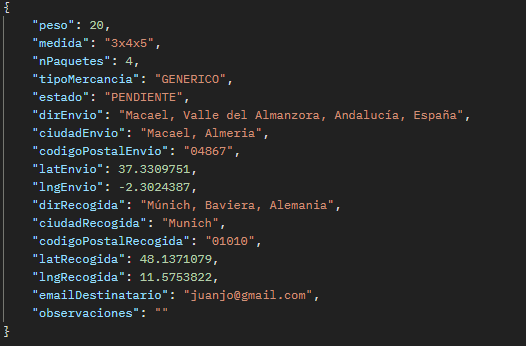
\includegraphics[width=0.7\textwidth]{imagenes/Implementacion/cuerpoPeticion.png}
    \caption{Cuerpo de la petición para crear una remesa}
    \label{fig:cuerpo_peticion_crear_remesa}
\end{figure}

Al recibir la petición el backend y procesarla, devolverá una respuesta con el estado
\texttt{201 Created} y el cuerpo de la respuesta incluirá los datos de la remesa creada en formato
JSON.
\begin{figure}[H]
    \centering
    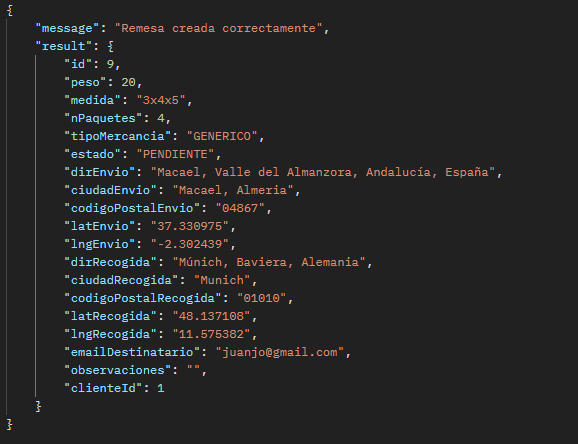
\includegraphics[width=0.7\textwidth]{imagenes/Implementacion/respuestaPeticionCorrecta.png}
    \caption{Cuerpo de la respuesta para crear una remesa}
    \label{fig:cuerpo_respuesta_crear_remesa}
\end{figure}

Si ha fallado la validación de los datos de entrada, el backend devolverá una respuesta con el estado
\texttt{400 Bad Request} y el cuerpo de la respuesta incluirá un mensaje de error.
\begin{figure}[H]
    \centering
    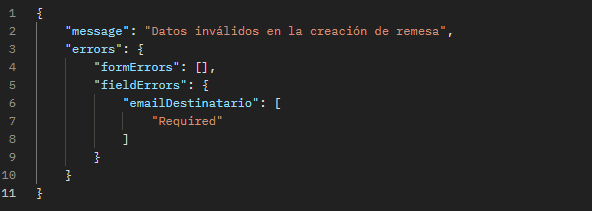
\includegraphics[width=0.7\textwidth]{imagenes/Implementacion/respuestaIncorrecta.png}
    \caption{Cuerpo de la respuesta incorrecta para crear una remesa}
    \label{fig:cuerpo_respuesta_incorrecta_crear_remesa}
\end{figure}

\subsection{Medidas de seguridad}
Para garantizar la seguridad del backend, se han implementado las siguientes medidas:
\begin{itemize}
    \item \textbf{Autenticación y autorización}: se utiliza JWT para autenticar a los usuarios y
    proteger los endpoints de la API REST. El flujo sería el siguiente:
    \begin{enumerate}
        \item El usuario envía una petición de inicio de sesión con sus credenciales.
        \item El backend verifica las credenciales y genera un token JWT si son correctas con la información
        del usuario que nos convenga (importante no incluir información sensible porque el token se puede decodificar y
        obtener su contenido ya que esta cifrado en base64) y una fecha de expiración.
        \item A partir de ese momento, el cliente debe incluir el token JWT en la cabecera de autorización de todas
        las peticiones a los endpoints protegidos.
        \item El backend verifica el token JWT en cada petición y permite o deniega el acceso.
    \end{enumerate}
    \item \textbf{Validación de datos}: se validan los datos de entrada en los controladores para
    evitar inyecciones SQL y otros ataques. Esto se consigue con la ayuda de librerías como \textit{Yup} y gracias a la ayuda
    de typeScript que permite definir tipos de datos estrictos. Si una validación falla automáticamente el backend responde 
    con un error \texttt{400 Bad Request}.
    \item \textbf{Cifrado de contraseñas}: Es importante almacenar las contraseñas de los usuarios de forma segura.
    Se utiliza la librería \textit{bcrypt} para hashear las contraseñas antes de almacenarlas en la base de datos.
    Es decir, se aplica una función hash que convierte la contraseña en una cadena de caracteres irreconocible.
    De esta forma, aunque un atacante consiga acceder a la base de datos, no podrá obtener las contraseñas originales.
    \item \textbf{Protección contra ataques XSS}: se implementan medidas para evitar la inyección y ejecución de scripts maliciosos tanto en el servidor como en el cliente:
        \begin{itemize}
        \item \textbf{Cabeceras de seguridad con Helmet}: se añaden cabeceras como 
        \textit{X-Content-Type-Options: nosniff}, 
        \textit{X-Frame-Options}, \textit{Referrer-Policy}, etc.
        \item \textbf{Respuestas como JSON}: todas las respuestas se sirven con \texttt{Content-Type: application/json}, evitando que el navegador las trate como HTML ejecutable.
        \item \textbf{Saneado de entradas}: se aplica un middleware que recorre \texttt{req.body} y \texttt{req.query} y limpia todas las cadenas con la librería \texttt{xss} antes de llegar a las rutas, mitigando cargas como \texttt{<script>} o atributos \texttt{onerror=} si posteriormente se renderizan en el cliente.
        \end{itemize}
\end{itemize}

\subsection{Algoritmo de planificación de rutas}
Para optimizar la asignación de transportistas a las remesas, se ha implementado un algoritmo Voraz que tiene en cuenta
la proximidad geográfica y la disponibilidad de los transportistas.\\

Primero tener en cuenta que para obtener las coordenadas geográficas cuando un usuario ingresa una dirección se ha utilizado la API de
\textit{LocationIQ}. \href{https://es.locationiq.com}{LocationIQ} es un servicio de geocodificación que permite convertir
direcciones en coordenadas geográficas (latitud y longitud) y viceversa entre otros servicios.\\

El algoritmo voraz funciona de la siguiente manera:
\begin{enumerate}
    \item Se hace una búsqueda en la base de datos de los transportistas disponibles con vehículo que puedan realizar el envío.
    \item Se calcula cuántos transportistas serán necesarios en función de la distancia que hay entre el punto donde se recoge la remesa y el punto donde se entrega.
    Se ha tenido en cuenta que un transportista solo puede conducir un máximo de 5 horas por día.
    \item Se selecciona en función de la distancia geográfica respecto a la remesa a enviar el transportista más cercano.
    \item Cada vez que se asigna un transportista se calcula el punto donde deberá entregar la remesa ya sea al cliente final o al siguiente transportista.
    \item Se repite el proceso hasta que se hayan asignado todos los transportistas necesarios.
\end{enumerate}
\begin{figure}[H]
    \centering
    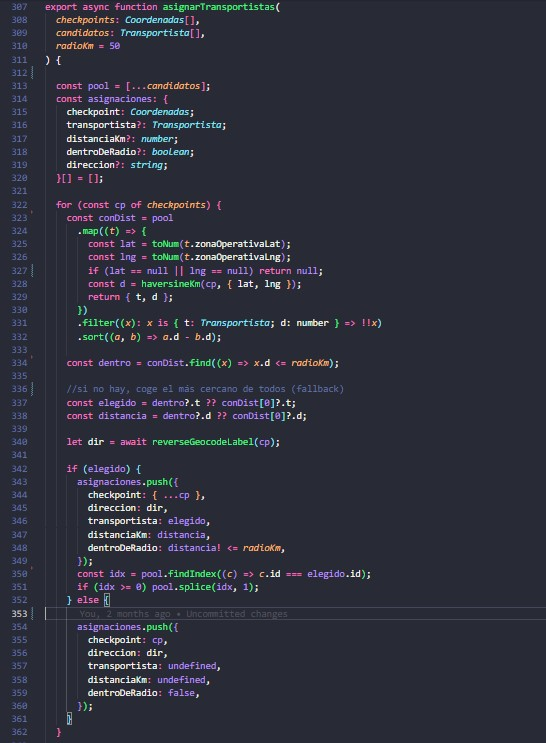
\includegraphics[width=0.7\textwidth]{imagenes/Implementacion/codigoImplementacionAsignarTransportistasARemesas.jpg}
    \caption{Código algoritmo}
    \label{fig:algoritmo_voraz_asignacion_transportistas}
\end{figure}

\section{Implementación del frontend}
\subsection{Arquitectura en el frontend}
El frontend de la aplicación web se ha desarrollado utilizando el framework \textit{React.js}, el desarrollo con React
se basa en la creación de componentes reutilizables que representan diferentes partes de la interfaz de usuario, desde un simple botón hasta
una página completa.\\

Estos componentes pueden tener su propio estado y propiedades, lo que permite una gran flexibilidad y modularidad en el desarrollo de la aplicación.\\

React facilita también la creación de interfaces de usuario interactivas y dinámicas
al permitir la actualización eficiente del DOM mediante un sistema de reconciliación
y un DOM virtual utilizado para comparar los cambios y actualizar las partes necesarias
de la interfaz de usuario sin necesidad de recargar toda la página.\\


\subsection{Estructura de carpetas}
\begin{figure}[H]
    \centering
    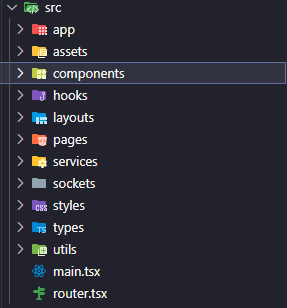
\includegraphics[width=0.7\textwidth]{imagenes/Implementacion/estructuraCarpetasFrontEnd.png}
    \caption{Estructura de carpetas del frontend}
    \label{fig:estructura_frontend}
\end{figure}

\begin{itemize}
\item \textbf{\texttt{src/services}}: Contiene los archivos referentes al manejo de estado global y las llamadas a las APIs.
\item \textbf{\texttt{src/components}}: componentes reutilizables de la interfaz de usuario. Se divide en subcarpetas según sea componentes comunes a construir interfaces de usuario mas complejas a partir de ellos
como por ejemplo botones, tablas, loaders, etc. o layouts que son componentes construidos 
a partir de estos comunes y que son utilizados en varias páginas como el navbar, footer,...
\item \textbf{\texttt{src/hooks}}: definición de los hooks personalizados. Se utilizan para encapsular la lógica de negocio y el estado de los componentes.
\item \textbf{\texttt{src/layout}}: componentes que definen la estructura común o general de una página. Aquí al ser un componente común por ejemplo a las páginas
de los usuarios que están autenticados, es una buena práctica introducir esta lógica en un layout.
\item \textbf{\texttt{src/pages}}: páginas de la aplicación. Cada página representa una vista completa de la aplicación. Por ejemplo la página de login, la página de gestionar remesas, etc.
\item \textbf{\texttt{src/sockets}}: lógica de comunicación en tiempo real mediante WebSockets. Es decir, la configuración
y manejo de eventos para la comunicación bidireccional entre el cliente y el servidor.
\item \textbf{\texttt{src/styles}}: Aquí se encuentran estilos predefinidos que tendrán todos los componentes para que la aplicación construida
tenga una apariencia coherente y uniforme.
\item \textbf{\texttt{src/types}}: Tipos de los datos que deben tener de las respuestas del backend para que haya una coherencia de tipos entre estas dos capas. 
\item \textbf{\texttt{src/utils}}: Funciones de ayuda para tareas comunes.
\end{itemize}

\subsection{Comunicación con el backend}
La comunicación entre el frontend y el backend se realiza a través de la API REST utilizando
la librería \hyperlink{https://redux-toolkit.js.org/rtk-query/overview}{Redux Toolkit Query}. Esta librería
se puede utilizar tanto para gestionar el estado global de la aplicación como para realizar
llamadas a APIs de manera sencilla y eficiente. \\

Esta librería permite a la hora de hacer llamadas a la api definir "slices" que son
conjuntos de endpoints relacionados entre sí. Por ejemplo, se ha definido un slice para
gestionar las remesas, otro para los usuarios, otro para los transportistas, etc.\\
\begin{figure}[H]
    \centering
    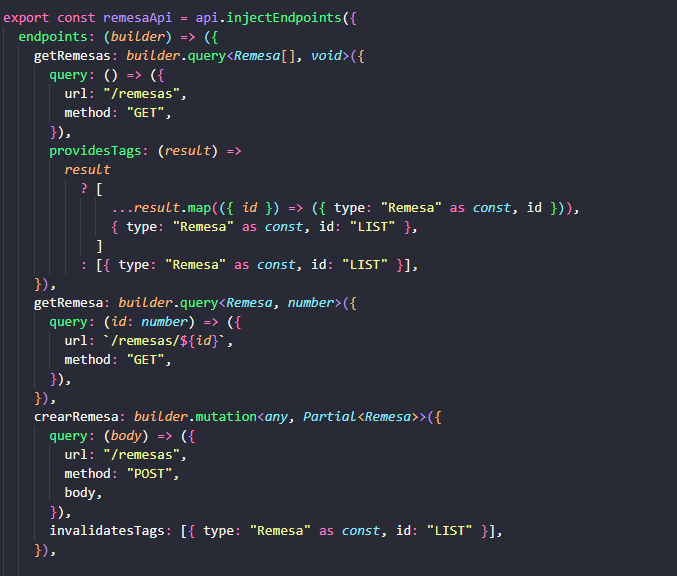
\includegraphics[width=0.7\textwidth]{imagenes/Implementacion/sliceRemesa.png}
    \caption{Definición de un slice con Redux Toolkit Query}
    \label{fig:definicion_slice_rtk}
\end{figure}

Además a la hora de mostrar la información en los componentes, te proporciona hooks
predefinidos para gestionar el estado de carga, error y datos de manera automática haciendose cargo
también de la caché de las respuestas y la asincronía de las llamadas facilitando mucho el desarrollo.


\subsection{Experiencia de usuario}
Para mejorar la experiencia de usuario en la aplicación web, se ha seguido el principio
de mobile-first, diseñando la interfaz de usuario para que sea accesible y funcional
en dispositivos móviles antes que en dispositivos de escritorio.\\

Se ha utilizado la librería \textit{Tailwind CSS} para facilitar el diseño responsivo
y la creación de estilos personalizados.\\

Se han elegido colores con contrastes y tipografías que mejoran la legibilidad y la usabilidad de la aplicación.
Además, se han implementado animaciones y transiciones suaves para mejorar la interacción.

\begin{figure}
    \centering
    
\includegraphics[width=0.7\textwidth]{imagenes/Implementacion/capturasPantalla/home.jpg}
    \caption{Interfaz de usuario del frontend (1/7)}
    \label{fig:interfaz_usuario_frontend_1}
\end{figure}

\begin{figure}
    \centering
    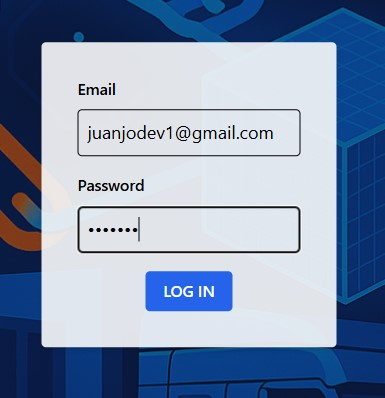
\includegraphics[width=0.7\textwidth]{imagenes/Implementacion/capturasPantalla/login.jpg}
    \caption{Interfaz de usuario del frontend (2/7)}
    \label{fig:interfaz_usuario_frontend_2}
\end{figure}

\begin{figure}
    \centering
    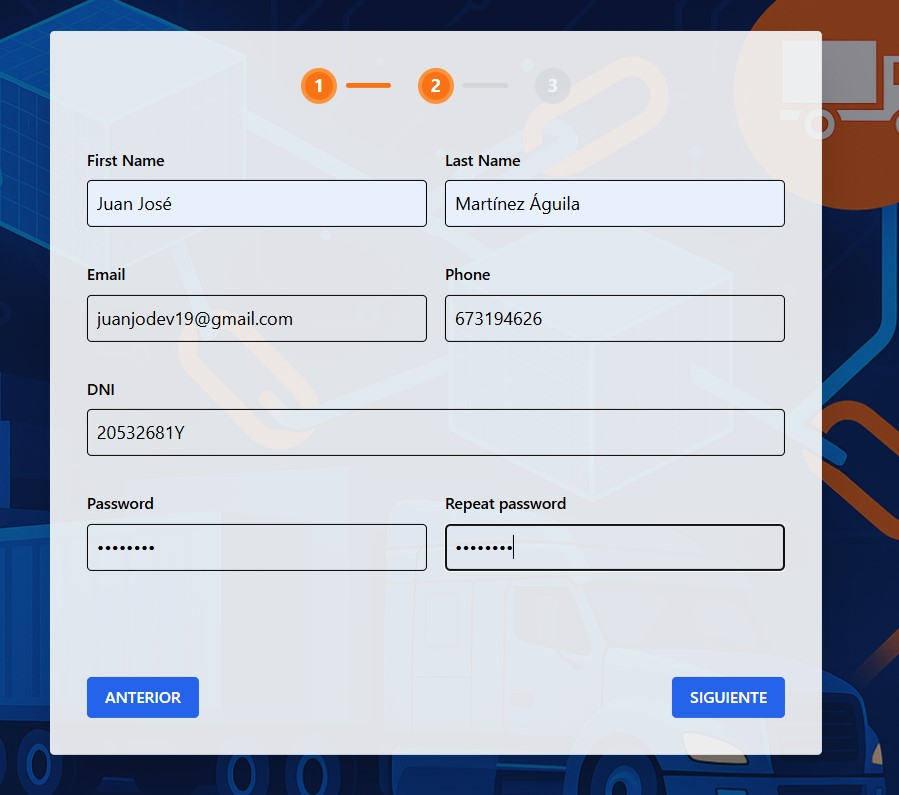
\includegraphics[width=0.7\textwidth]{imagenes/Implementacion/capturasPantalla/register.jpg}
    \caption{Interfaz de usuario del frontend (3/7)}
    \label{fig:interfaz_usuario_frontend_3}
\end{figure}

\begin{figure}
    \centering
    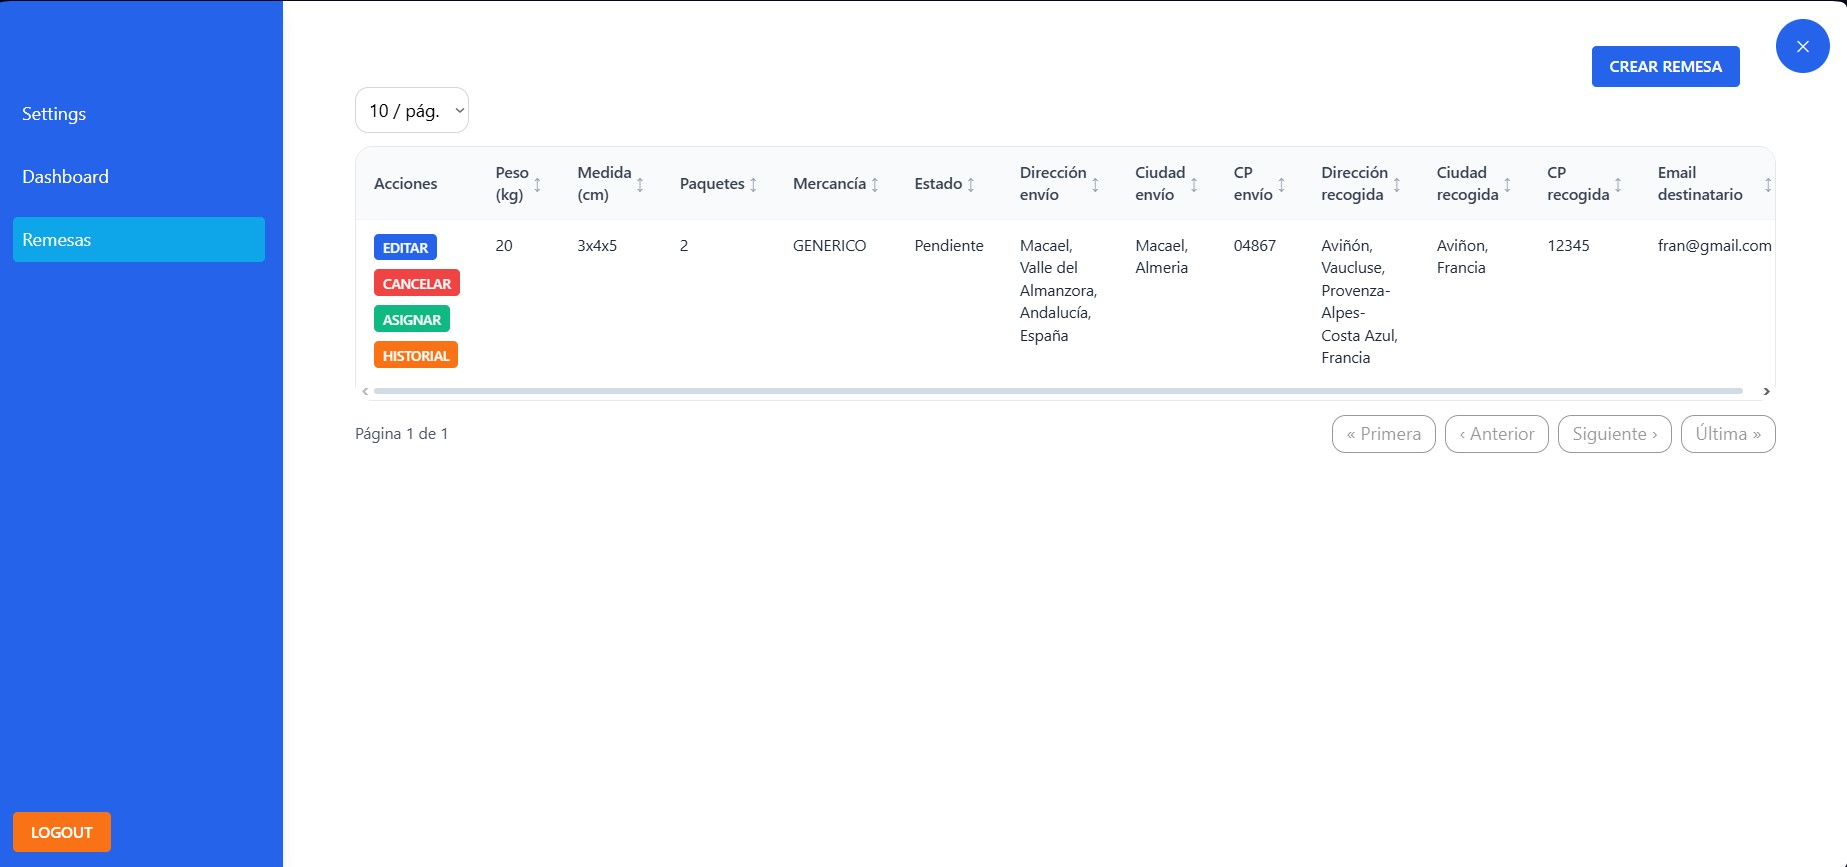
\includegraphics[width=0.7\textwidth]{imagenes/Implementacion/capturasPantalla/remesas.jpg}
    \caption{Interfaz de usuario del frontend (4/7)}
    \label{fig:interfaz_usuario_frontend_4}
\end{figure}

\begin{figure}
    \centering
    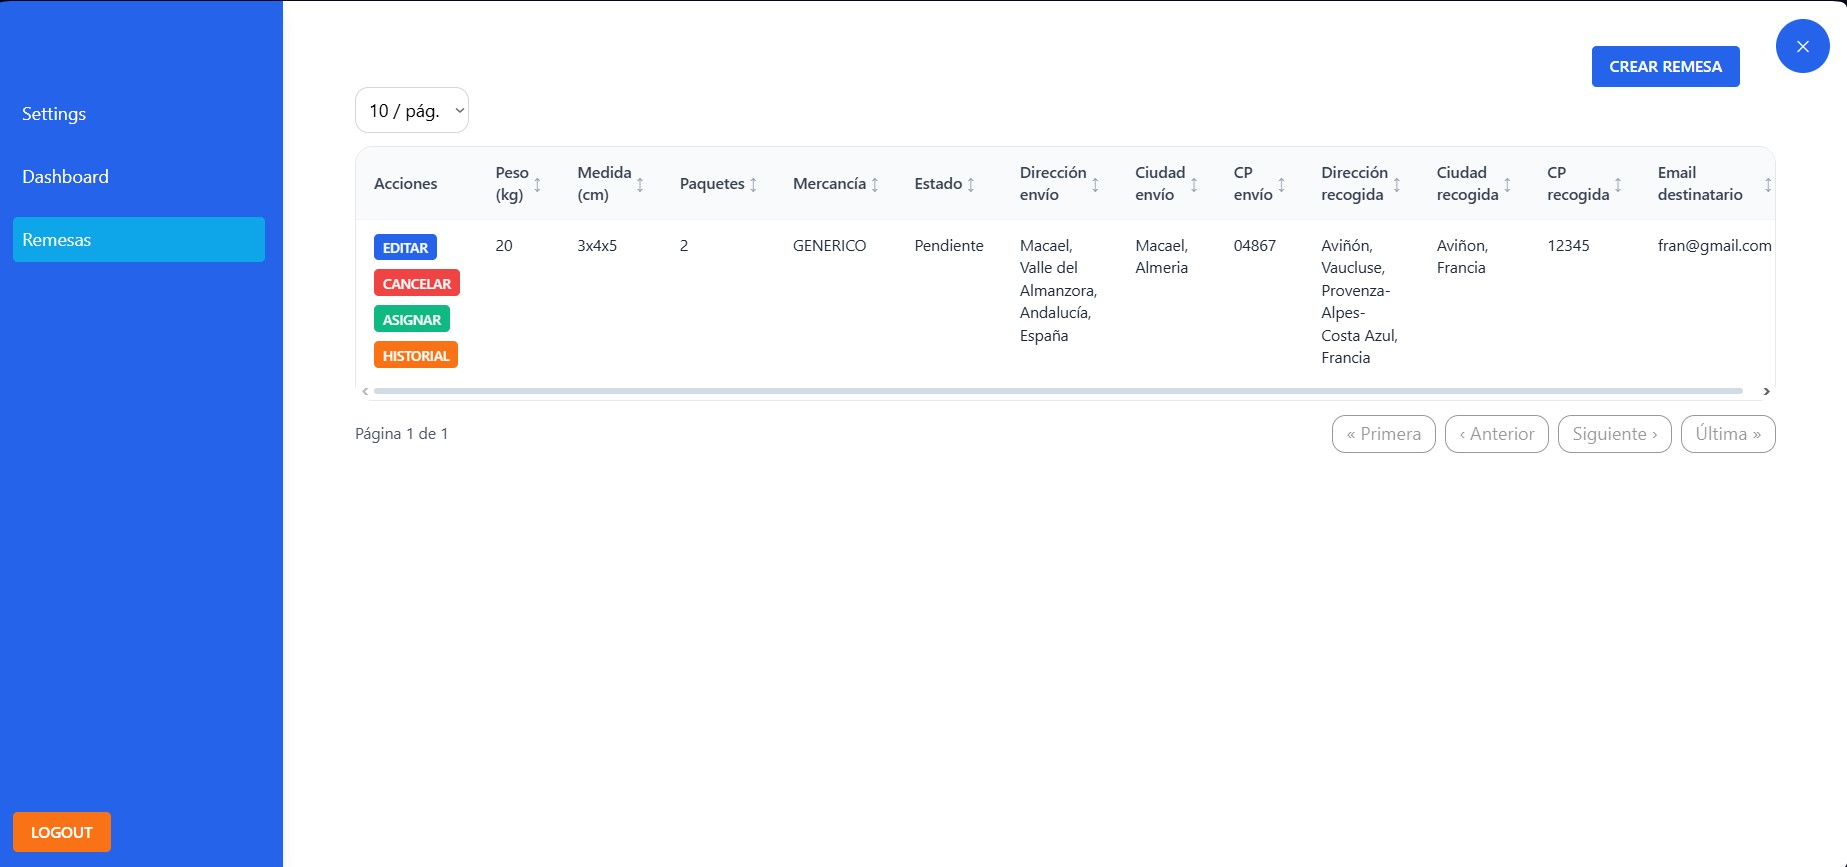
\includegraphics[width=0.7\textwidth]{imagenes/Implementacion/capturasPantalla/remesas.jpg}
    \caption{Interfaz de usuario del frontend (5/7)}
    \label{fig:interfaz_usuario_frontend_5}
\end{figure}

\begin{figure}
    \centering
    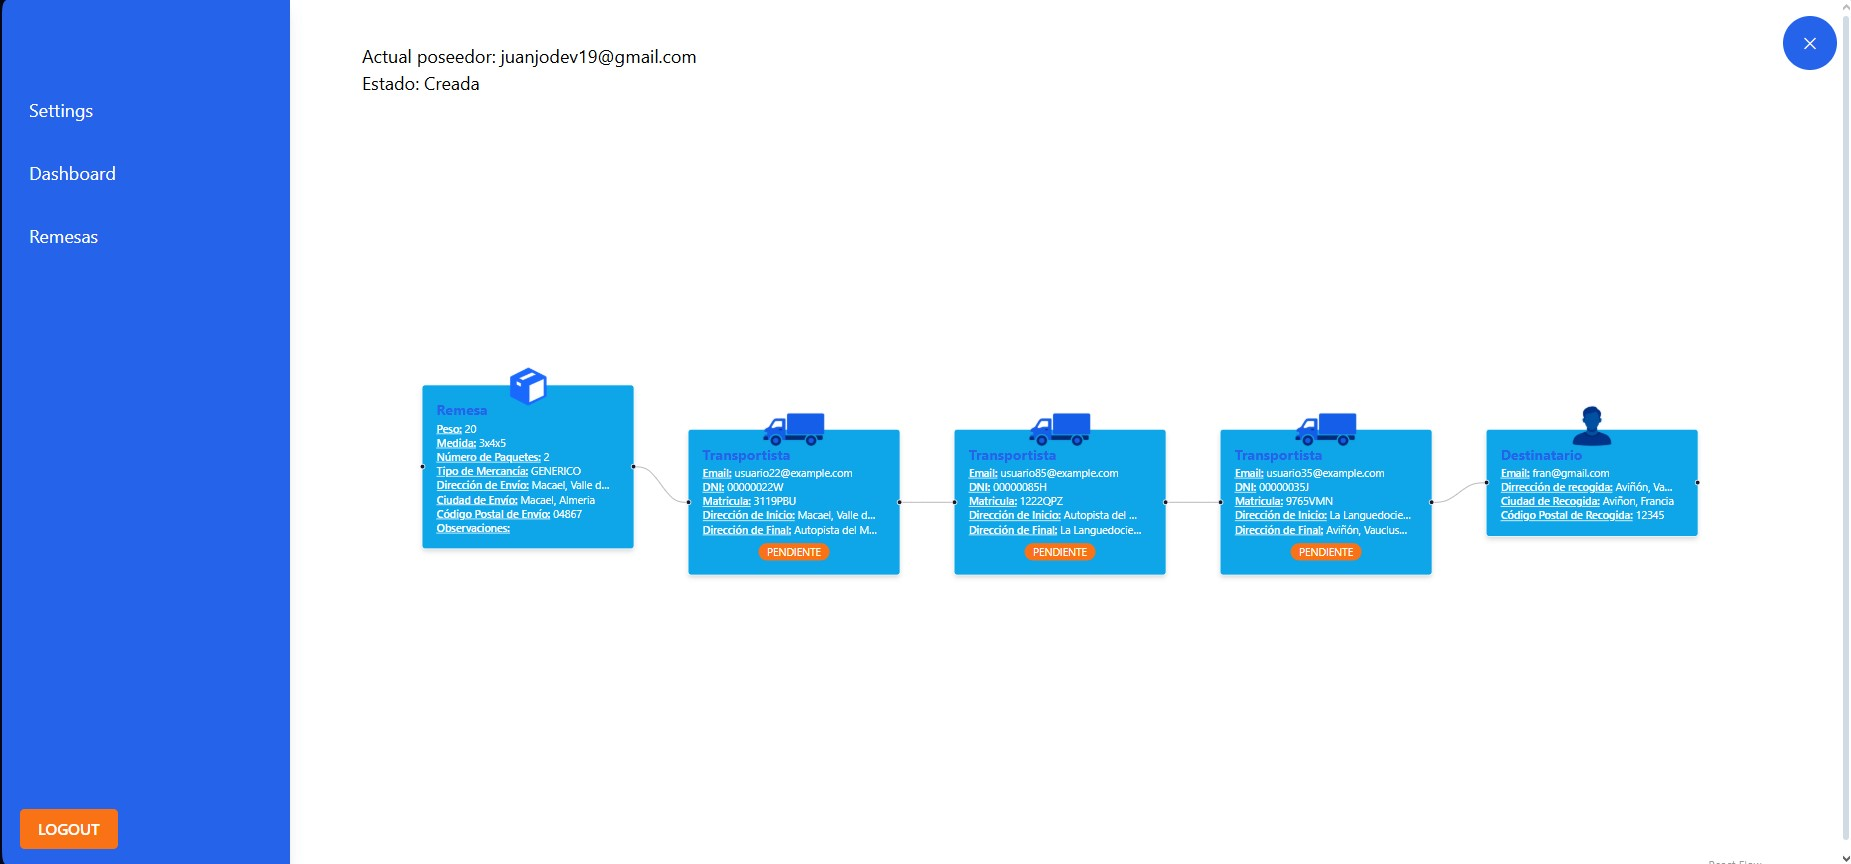
\includegraphics[width=0.7\textwidth]{imagenes/Implementacion/capturasPantalla/seguimientoEnvio.jpg}
    \caption{Interfaz de usuario del frontend (6/7)}
    \label{fig:interfaz_usuario_frontend_6}
\end{figure}
\begin{figure}
    \centering
    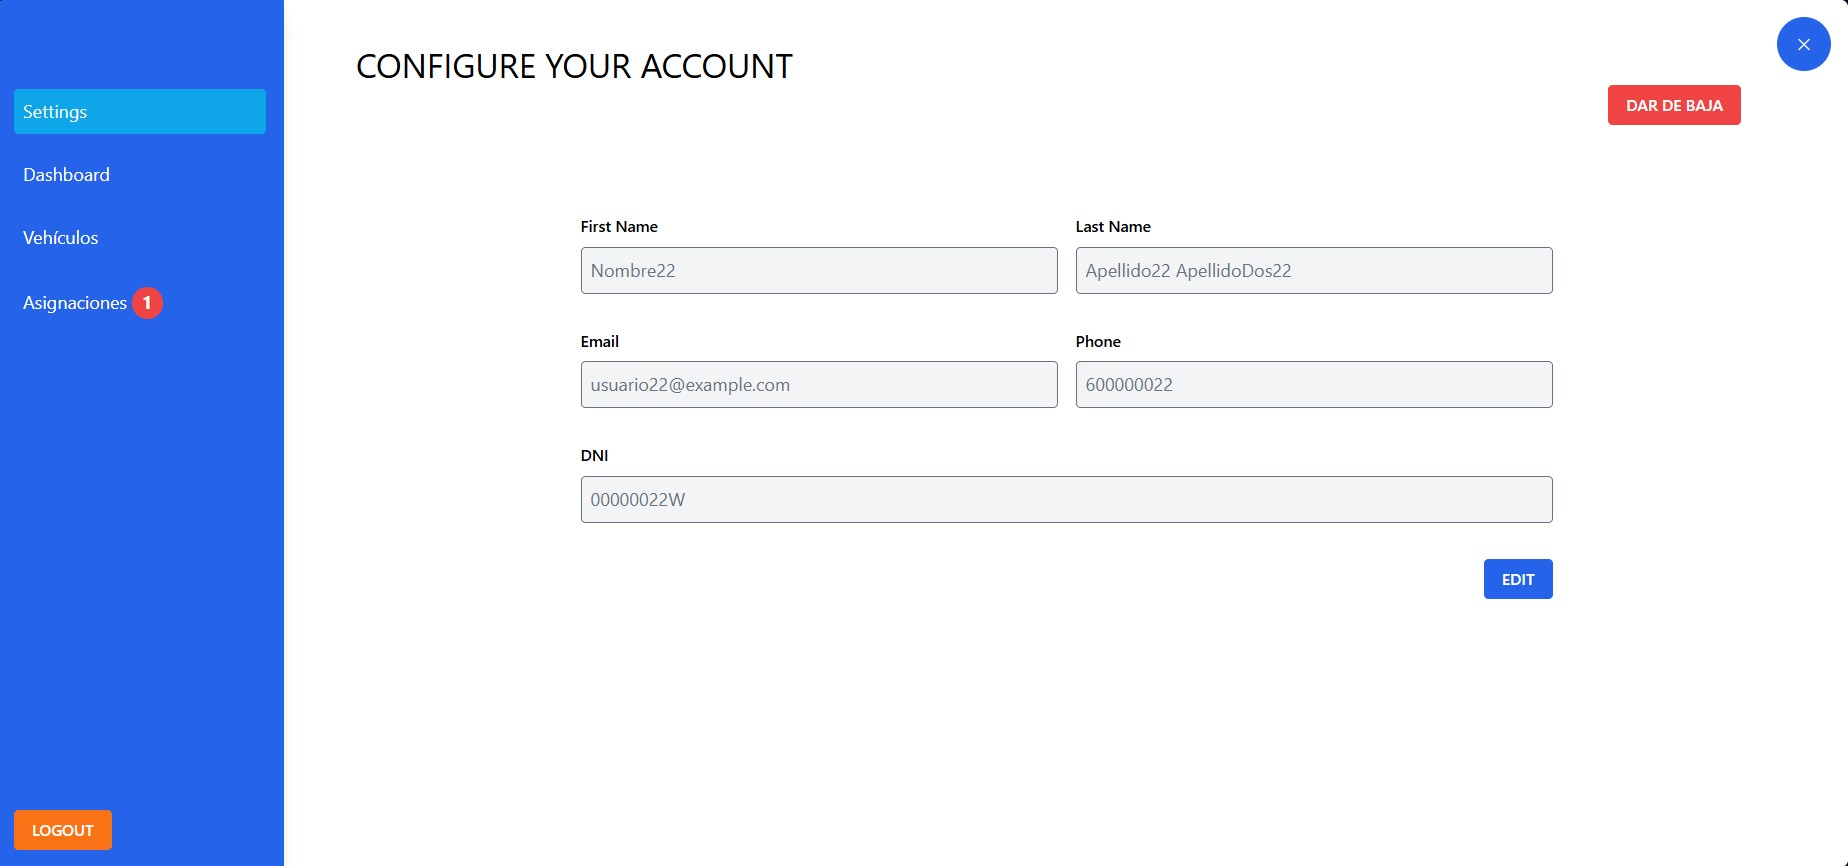
\includegraphics[width=0.7\textwidth]{imagenes/Implementacion/capturasPantalla/transportistaMenu.jpg}
    \caption{Interfaz de usuario del frontend (7/7)}
    \label{fig:interfaz_usuario_frontend_6}
\end{figure}




\subsection{Rendimiento}
Para optimizar el rendimiento del frontend, se han implementado las siguientes técnicas:
\begin{itemize}
    \item \textbf{Carga diferida (lazy loading)}: se ha implementado la carga diferida de componentes
    y recursos para reducir el tiempo de carga inicial de la aplicación. Esto significa que
    los componentes y recursos se cargan solo cuando son necesarios, mejorando la velocidad
    de la aplicación.
    \item \textbf{Optimización de imágenes}: se han utilizado formatos de imagen modernos como
    WebP y se han comprimido las imágenes para reducir su tamaño sin perder calidad.
    \item \textbf{Optimización de re-renders}: En React, cada vez que se detecta que ha habido un cambio
    en el estado se realizan los llamados re-renders para actualizar la interfaz de usuario. Estos rerenders se producen
    desde el componente raíz donde se produce el cambio del estado hasta todos los componentes hijos aunque 
    no tengan la necesidad de actualizarse. Para evitar estos re-renders se han utilizado técnicas y/o patrones de diseño
    para extraer todos los componentes que tengan un estado propio que no debería afectar a otros y se les ha separado a un componente independiente de los hijos
    para que solo se rendericen cuando su propio estado cambie mejorando así el rendimiento.
\end{itemize}

\section{Red Ethereum}
La red Ethereum se encarga de almacenar la información de trazabilidad y autenticidad
de las remesas de manera segura y descentralizada.\\
Para interactuar con la red Ethereum, se ha utilizado la librería \textit{ethers.js}, que
permite crear y gestionar contratos inteligentes de manera sencilla.\\

Se ha decidido utilizar la red de pruebas \textit{Hardhat} en lugar de la red principal de Ethereum, 
con el fin de evitar los costes asociados a las transacciones reales y facilitar el proceso de desarrollo, depuración y validación de la aplicación. 
Ya que para el desarrollo hay que tener en cuenta que cada vez que se realiza una transacción en
la red Ethereum, se incurre en un coste llamado \textit{gas}, que se paga en \textit{Ether} (ETH).\\

Una red como \textit{Hardhat} permite simular localmente el funcionamiento de una red blockchain,
 reproduciendo el comportamiento de una red descentralizada pero sin requerir la participación de nodos externos. 
 De este modo, se pueden realizar pruebas y despliegues de contratos inteligentes de forma rápida y controlada,
 manteniendo la lógica de ejecución de Ethereum sin incurrir en los costes ni la latencia de una red pública.\\

Una alternativa sería haber utilizado otra red de pruebas como \textit{Sepolia} que a diferencia
de \textit{Hardhat} es una red pública y descentralizada y no una red local. Pero para poder utilizarla
necesitas que te den ETH de prueba a través de faucets, lo cual puede ser un proceso lento y tedioso.\\

Un faucet es un servicio que proporciona pequeñas cantidades de criptomonedas de prueba de forma
gratuita a los desarrolladores y usuarios que desean probar aplicaciones en una red de pruebas.\\

\subsubsection{Flujo de desarrollo de un contrato inteligente}
A la hora de desarrollar un contrato inteligente, primero se ha realizado desde un entorno en la nube
llamado \textit{Remix IDE}, que permite escribir, compilar y desplegar contratos inteligentes.\\
Se ha desarrollado el contrato inteligente en \textit{Remix IDE} para probar su funcionalidad
y corregir errores antes de integrarlo en el backend de una manera sencilla ya que Remix IDE te proporciona
una interfaz gráfica para interactuar con el contrato inteligente desplegado y una red local para
probarlo sin necesidad de desplegarlo en una red pública.\\

\begin{figure}[H]
    \centering
    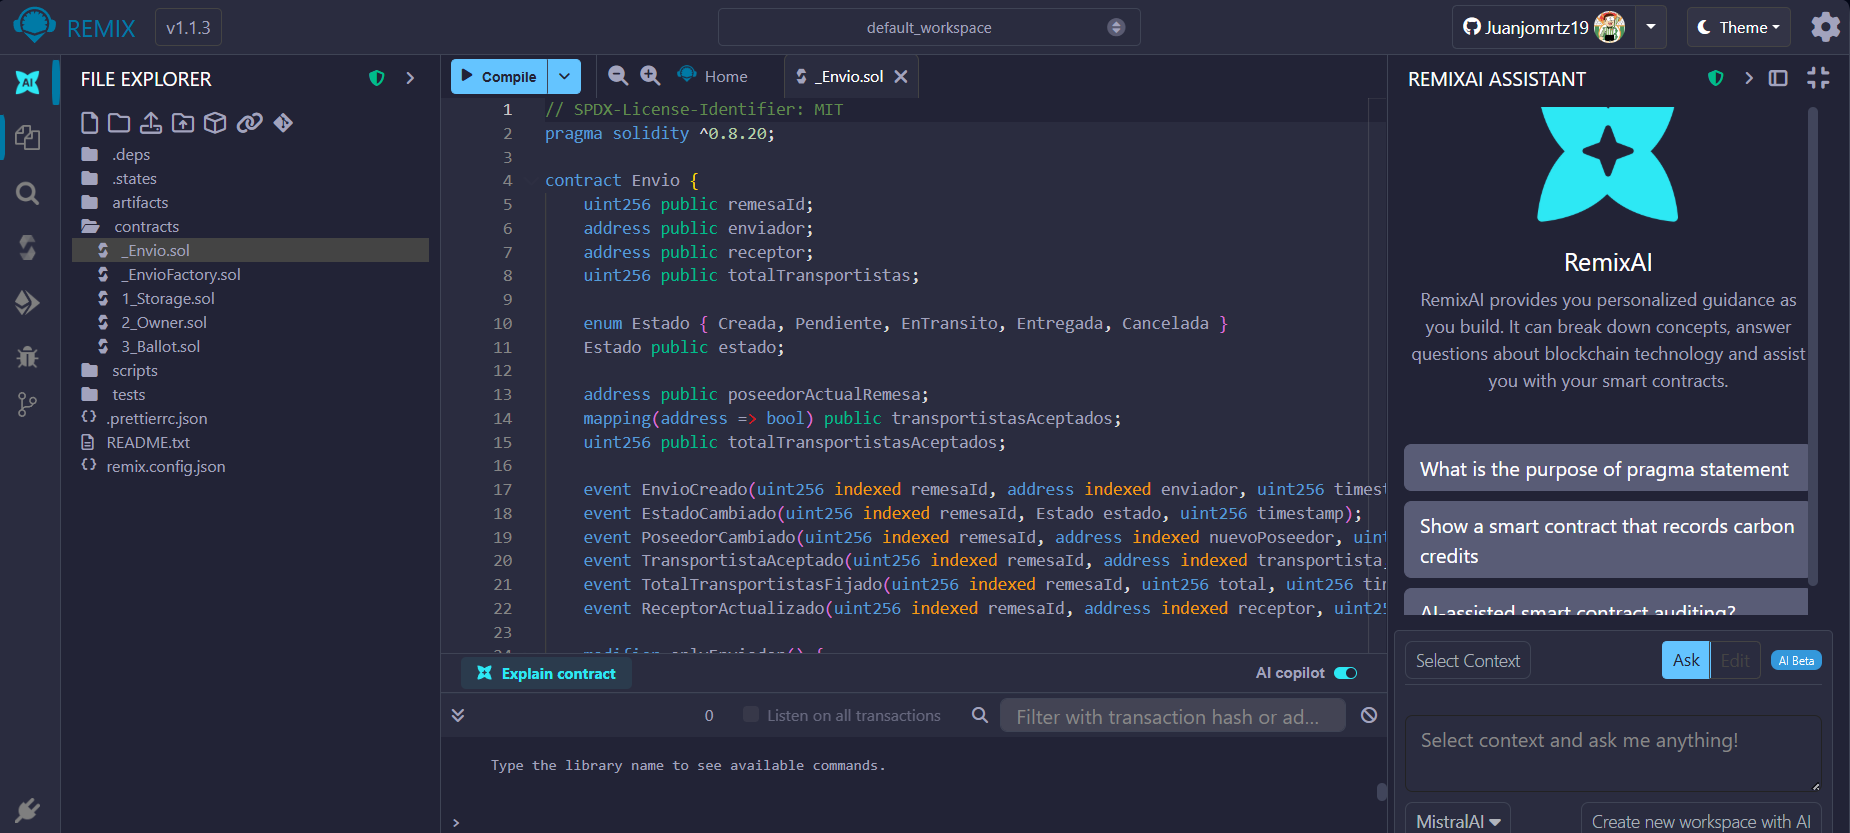
\includegraphics[width=0.7\textwidth]{imagenes/Implementacion/entornoRemix.png}
    \caption{Interfaz de Remix IDE para desarrollar contratos inteligentes}
    \label{fig:remix_ide}
\end{figure}

Una vez el contrato inteligente ha sido probado y corregido, es hora de pasarlo al código del
proyecto. Para ello necesitamos pasar el código del contrato inteligente a un archivo \textit{.sol}.
Luego, se crearán los test para testear el contrato inteligente utilizando librerías javascript como Mocha.\\

\begin{figure}[H]
    \centering
    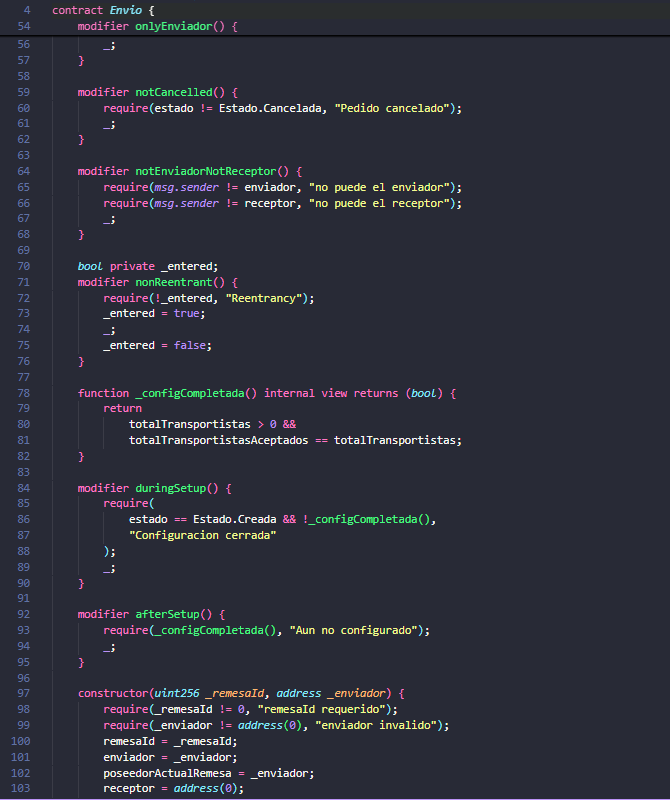
\includegraphics[width=0.7\textwidth]{imagenes/Implementacion/contratoInteligente.png}
    \caption{Código contrato inteligente en archivo .sol}
    \label{fig:test_contrato_inteligente}
\end{figure}

Finalmente, habrá que programar dos scripts para compilar y desplegar el contrato inteligente. 

\begin{itemize}
    \item \textbf{Compilación}: Cuando un contrato inteligente es compilado, se genera un archivo JSON que contiene el \textit{ABI} (Application Binary Interface) y el bytecode del contrato
inteligente. El \textit{ABI} es una descripción del contrato inteligente que permite a las aplicaciones interactuar
con él, mientras que el bytecode es el código binario que se ejecuta en la máquina virtual de Ethereum.
\begin{figure}[H]
    \centering
    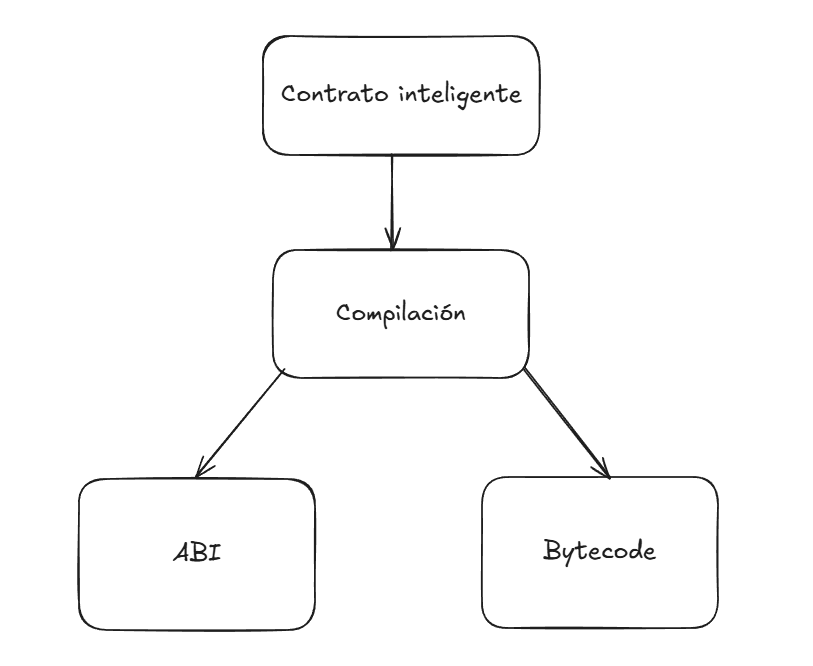
\includegraphics[width=0.7\textwidth]{imagenes/Implementacion/esquemaCompilacion.png}
    \caption{Esquema compilación contrato inteligente}
    \label{fig:script_despliegue_contrato_inteligente}
\end{figure}
El script de compilación funcionaría de la siguiente manera:
\begin{enumerate}
\item \textbf{Listar los contratos inteligentes}: listar los ficheros \texttt{.sol} de la carpeta donde están alojados los contratos inteligentes.
\item \textbf{Construir el objeto de entrada}: construir un objeto de entrada para el compilador Solidity con los archivos listados.
\item \textbf{Configurar opciones de compilación}: configurar las opciones de compilación.
\item \textbf{Resolver dependencias}: resolver \textit{imports} locales y de \textit{node modules}, ya que al compilar con \texttt{solc} no tiene acceso al disco y necesita que los \textit{imports} se resuelvan previamente.
\item \textbf{Compilar los contratos}: compilar los contratos inteligentes utilizando el compilador \texttt{Solc}.
\item \textbf{Guardar resultados}: guardar el \textit{output} de la compilación en archivos \texttt{JSON} en la carpeta de \texttt{build}.
\end{enumerate}

Los outputs de la compilación es lo que se utilizará a nivel de la lógica de la aplicación para interactuar con el
contrato inteligente y a su vez con la red Ethereum.

\item \textbf{Despliegue}: Se denomina a despliegue al proceso de subir el contrato inteligente a la red Ethereum. Este
proceso implica enviar una transacción a la red que contiene el bytecode del contrato inteligente.\\
El script de despliegue funcionaría de la siguiente manera:
\begin{enumerate}
\item \textbf{Configurar el proveedor RPC local}: inicializar un \textit{JsonRpcProvider} apuntando al nodo de Hardhat en \texttt{http://127.0.0.1:8545}
.
\item \textbf{Importar el artefacto del contrato}: cargar el JSON compilado de \textit{EnvioFactory} (contiene \texttt{abi} y \texttt{bytecode}).
\item \textbf{Validar artefacto}: comprobar que el JSON importado incluye \texttt{abi} y \texttt{bytecode}; en caso contrario, abortar con un error descriptivo.
\item \textbf{Inicializar la cuenta de despliegue}: crear un \textit{Wallet} de \texttt{ethers} usando una clave privada de las cuentas del nodo de Hardhat y asociarlo al proveedor.
\item \textbf{Construir la fábrica de contratos}: crear un \textit{ContractFactory} con la \texttt{abi}, el \texttt{bytecode} y el \textit{wallet} para firmar y enviar transacciones.
\item \textbf{Desplegar el contrato}: invocar \texttt{factory.deploy()} (sin argumentos al no tener constructor con parámetros) para enviar la transacción de despliegue.
\item \textbf{Esperar la inclusión en bloque}: llamar a \texttt{waitForDeployment()} para bloquear la ejecución hasta que el contrato quede minado y disponible en la red local.
\item \textbf{Obtener la dirección del contrato}: recuperar la dirección on-chain mediante \texttt{contract.getAddress()}.
\item \textbf{Preparar la salida para clientes}: construir la ruta \texttt{deployments/localhost} en el proyecto y crear la carpeta si no existe.
\item \textbf{Persistir metadatos de despliegue}: guardar un archivo \texttt{EnvioFactory.json} con la \texttt{address}, la \texttt{abi} y el identificador de \texttt{network} para que frontend/backend puedan conectarse al contrato.
\end{enumerate}

\end{itemize}

\subsection{Interacción del backend con la red blockchain desde las APIs}
\subsubsection{Flujo general de un endpoint}
\begin{enumerate}
\item \textbf{Inicialización del proveedor y cuenta de servicio}: el backend crea un \textit{provider} JSON-RPC (p.,ej., \texttt{http://127.0.0.1:8545}
 en Hardhat) y asocia un \textit{wallet} de servicio para firmar transacciones cuando sea necesario.
\item \textbf{Carga del contrato}: se importa el artefacto del contrato (\texttt{ABI}) y se instancia el contrato con \texttt{ethers} usando la dirección desplegada.
\item \textbf{Operaciones de lectura (\textit{call})}: los endpoints que consultan trazabilidad, estados o direcciones utilizan llamadas \textit{view/pure} sin coste de gas y sin firma.
\item \textbf{Operaciones de escritura (\textit{send})}: los endpoints que modifican estado (crear envío, actualizar estado, transferir posesión, etc.) preparan y firman una transacción con una cuenta autorizada (o con la cuenta del propio usuario, según el modelo elegido) y esperan el \textit{receipt}.
\item \textbf{Gestión de eventos}: tras minado, se leen eventos emitidos por el contrato (p.,ej., \texttt{EnvioCreado}, \texttt{EnvioEstadoActualizado}) para registrar metadatos y facilitar auditoría/observabilidad en la base de datos off-chain.
\item \textbf{Persistencia y respuesta}: el backend persiste lo necesario y responde al cliente con la información relevante.
\end{enumerate}

\subsection{Asignación de dirección blockchain por usuario}
\subsubsection{Motivación}
Para identificar de forma inequívoca a cada participante en la capa on-chain, la plataforma asocia a cada usuario una \textbf{dirección (address) blockchain}. Esta dirección se utiliza como identificador en los contratos inteligentes y como emisor/actor en las transacciones que afecten a la trazabilidad.

\subsubsection{Modelo aplicado en el entorno de desarrollo}
En el entorno de pruebas (Hardhat), se emplean \textbf{wallets ficticias} para simplificar la experiencia:
\begin{enumerate}
\item \textbf{Registro de usuario}: al crear el usuario en base de datos, se deriva/asigna un índice de wallet y se calcula su \textbf{address} correspondiente (p.,ej., mediante derivación determinista o a partir de cuentas del nodo local).
\item \textbf{Persistencia}: se guarda en la tabla de usuarios el \texttt{walletIndex} y la \texttt{walletAddress} en minúsculas.
\item \textbf{Fondeo opcional}: se intenta fondear la dirección con ETH de prueba para permitir transacciones firmadas en la red local (\textit{faucet} interno). Si falla, no se bloquea el registro.
\end{enumerate}

\subsubsection{Descripción del flujo }
\begin{enumerate}
\item \textbf{Creación del usuario y entidad dependiente}: se crea la fila en \texttt{usuario} y, según el rol, se crea \texttt{cliente} o \texttt{transportista} dentro de una transacción de base de datos.
\item \textbf{Derivación de dirección}: se calcula un \texttt{walletIndex} (p.,ej., \texttt{id-1}) y, con una función utilitaria (\texttt{addressFromIndex}), se obtiene la \texttt{walletAddress}.
\item \textbf{Vinculación en BD}: se actualiza el usuario con \texttt{walletIndex} y \texttt{walletAddress}.
\item \textbf{Fondeo de pruebas}: se invoca \texttt{ensureFunds(address, min, target)} para garantizar saldo mínimo en la red local; los errores no interrumpen el registro.
\end{enumerate}

\subsubsection{Consideraciones de seguridad y despliegue real}
\begin{itemize}
\item \textbf{Entorno de desarrollo}: es válido asignar \textbf{wallets ficticias} y, si procede, custodiar claves en local para automatizar pruebas.
\item \textbf{Producción (recomendado)}: evitar la custodia de claves privadas por el servidor. Preferir un modelo \textbf{no custodial} (el usuario firma con su propia wallet) o emplear \textbf{meta-transacciones/relayers} para mejorar la UX sin custodiar claves.
\item \textbf{Trazabilidad}: la address se usa como identificador on-chain; cualquier acción relevante (crear envío, cambio de estado, transferencia de posesión) debe asociarse a la address del actor.
\end{itemize}

\section{Estadísticas de la implementación}
A continuación se presentan algunas estadísticas relevantes sobre la implementación del proyecto como líneas de código, número de archivos, comentarios, etc.
\begin{figure}[H]
    \centering
    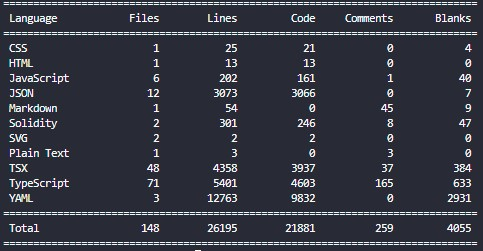
\includegraphics[width=0.7\textwidth]{imagenes/Implementacion/estadisticas.jpg}
    \caption{Estadísticas de la implementación}
    \label{fig:estadisticas_implementacion}
\end{figure}